\documentclass[a4paper]{article}
\usepackage{graphicx}
\usepackage{onecolpceurws}
\usepackage[utf8]{inputenc}

\title{Collaboration Networks in Software Development: Perspectives from Applying different Granularity Levels using Social Network Analysis - Research in Progress}

\author{
Miguel Ángel Fernández \\ GSyC/LibreSoft \\
                Universidad Rey Juan Carlos \\ ma.fernandezsa@alumnos.urjc.es
\and
Gregorio Robles \\ GSyC/LibreSoft \\
                Universidad Rey Juan Carlos \\ grex@gsyc.urjc.es
\and
Jesús M. González Barahona \\ Bitergia \\
                jgb@bitergia.com
}

\institution{}


\begin{document}
\maketitle

\vskip 32pt


\section{Introduction/Motivation}

Most social network studies for software projects are focused in a file-based
data of interactions in that network of developers. If there is a
collaboration between two or more developers in same file, how can we be sure
when there are thousands of lines of code if that people did actually
collaborate?

We want to go to a deeper level: in this particular case, a method-based
analysis which allows us to know with more accuracy if there is a real
relationship between those developers.

\section{Methodology}

The program studies registered changes made in a given repository tracked by
Git. From that repository, it extracts log from a specified date range. Using
that data, the program iterates with each commit made, and does a checkout
with all of them to take the repository to the state the program was when each
commit was made. At each iteration, we use Ctags with each file to get
classified all changes made in each of those files.

Next, is to find matches
between the commits information and Ctags data (still for each checkout), so
we can tell if a method has been modified.

Once the program finishes all checkout iterations, it takes that data and
searches for coincidences when different developers have modified same file
and method and outputs that data into two CSV-format files, one for in-file
collaborations and the other one for in-method collaborations; which can be
used in programs like Gephi to watch a graph-type representation of the
network.

\section{Case study: GNOME Gedit}

We used the program to study the evolution of GNOME-text editor Gedit (https://github.com/GNOME/gedit).

The considered date range for this study goes from the very beginning of
the project (At least, from the moment when log starts), which is April
15, 1998 until April 15, 2015.

\subsection{Results}

With this wide range of time, we have chosen time-lapses of six months so
we can handle and understand better the resulting data and its evolution
through these years.\\
First selected date range was from January 1, 2001 to May 31, 2001 
(First-half of year 2001) and second one was from June 1, 2014 to December
31, 2014 (Second-half of year 2014).\\

All this data, is represented in two different ways:\\
First one is a graphic representation of collaboration networks between
developers. Each node represents a developer, and edges represents
interactions between them.\\
We have two different graphs for each date range: an in-file collaboration
network (Developers who have modified same file) and an in-method
collaboration network (Developers who have modified same method).\\
\\
Second one is a numerical representation, particularly of an statistic
parameter referred to networks: Betweenness centrality.\\
The betweenness centrality of a node reflects the amount of control that
this node exerts over the interactions of other nodes in the network.\\

\subsubsection{Graphic results}

Figure 1 shows the different graphs (In-file and In-method data) from
first-half of 2001.

\begin{figure}[ht]
\begin{center}
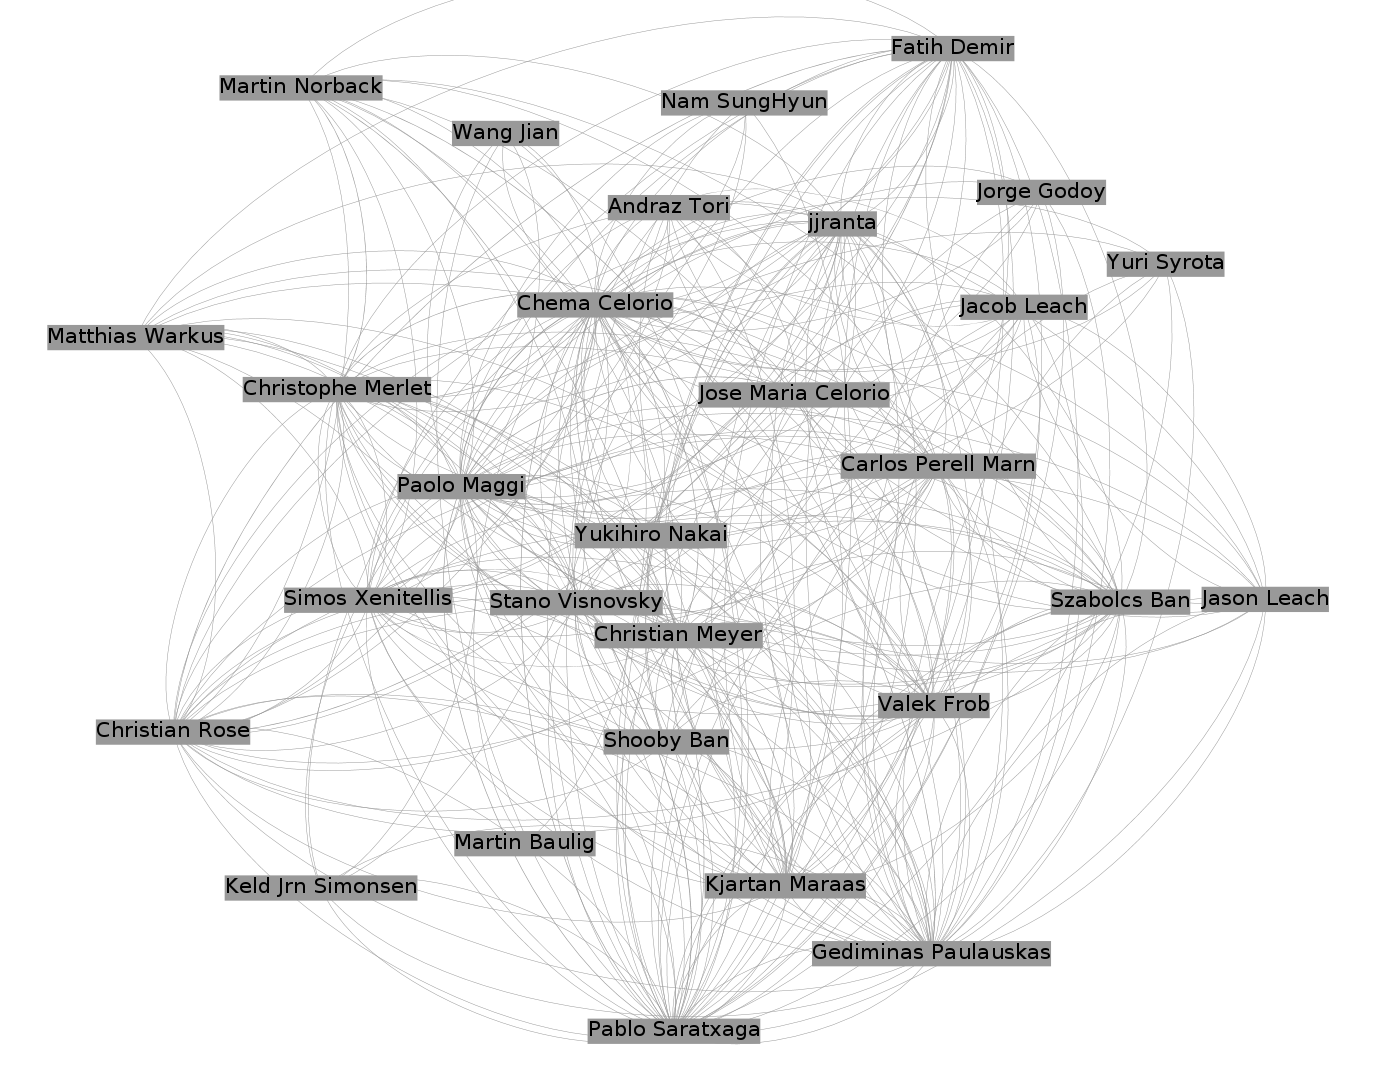
\includegraphics[scale=0.17]{g2001files.png} 
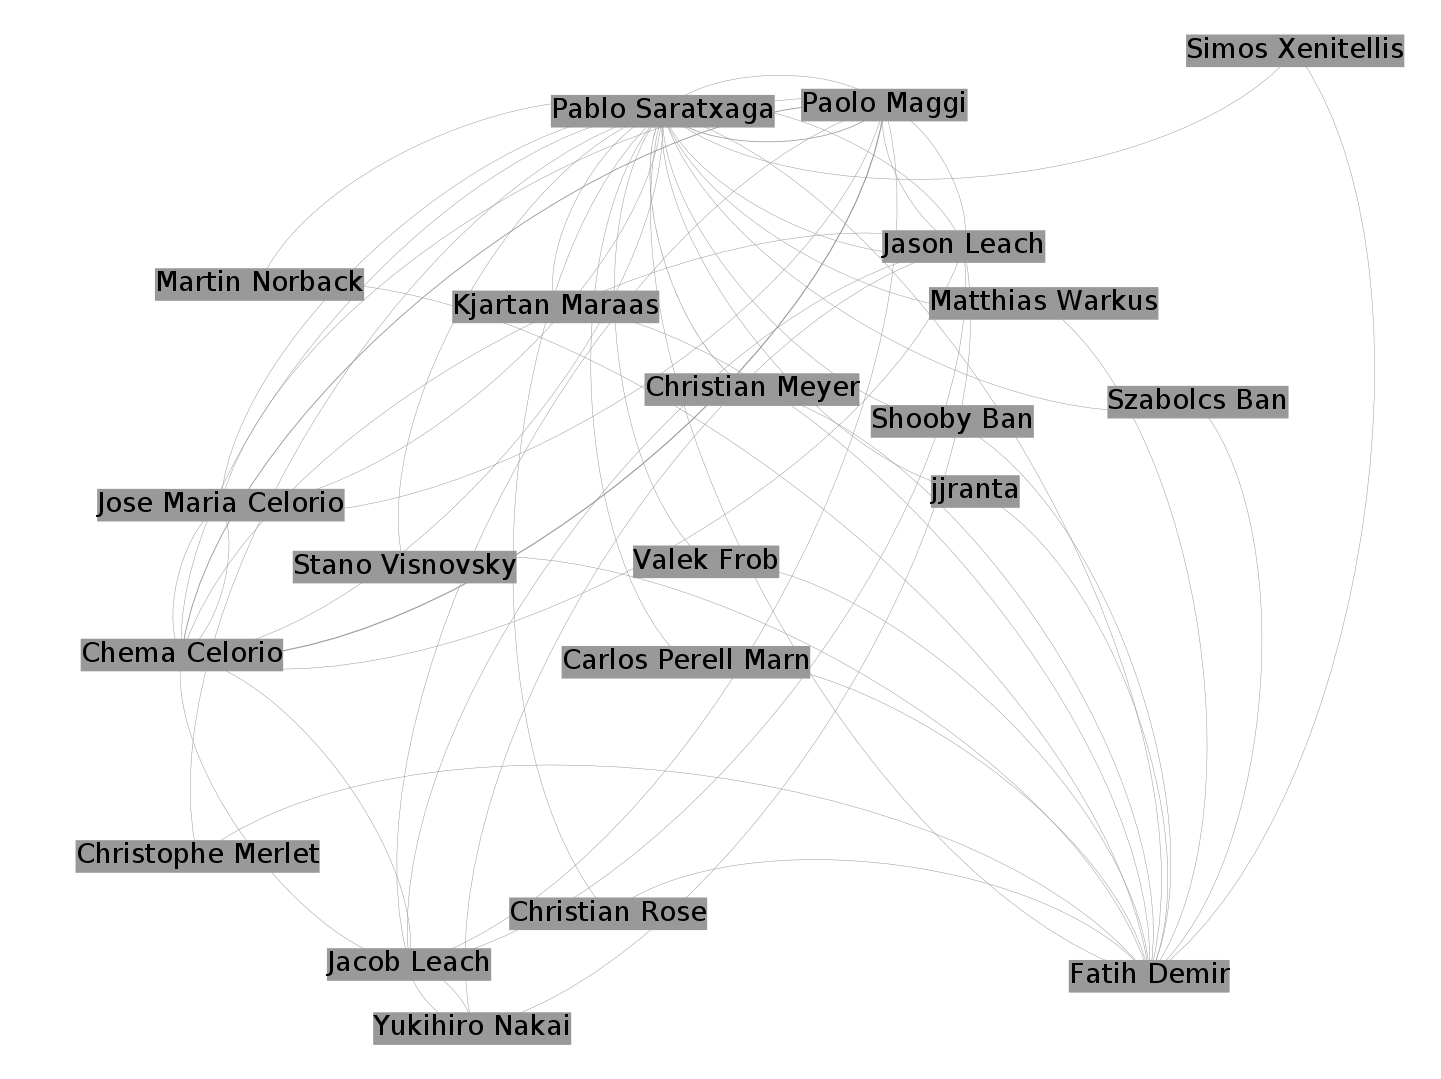
\includegraphics[scale=0.17]{g2001methods.png}
\caption{In-file (left) and In-method (right) collaboration graphs - 2001}
\label{fig:fixme1}
\end{center}
\end{figure}

Figure 2 shows the different graphs (In-file and In-method data) from
second-half of 2014.

\begin{figure}[ht]
\begin{center}
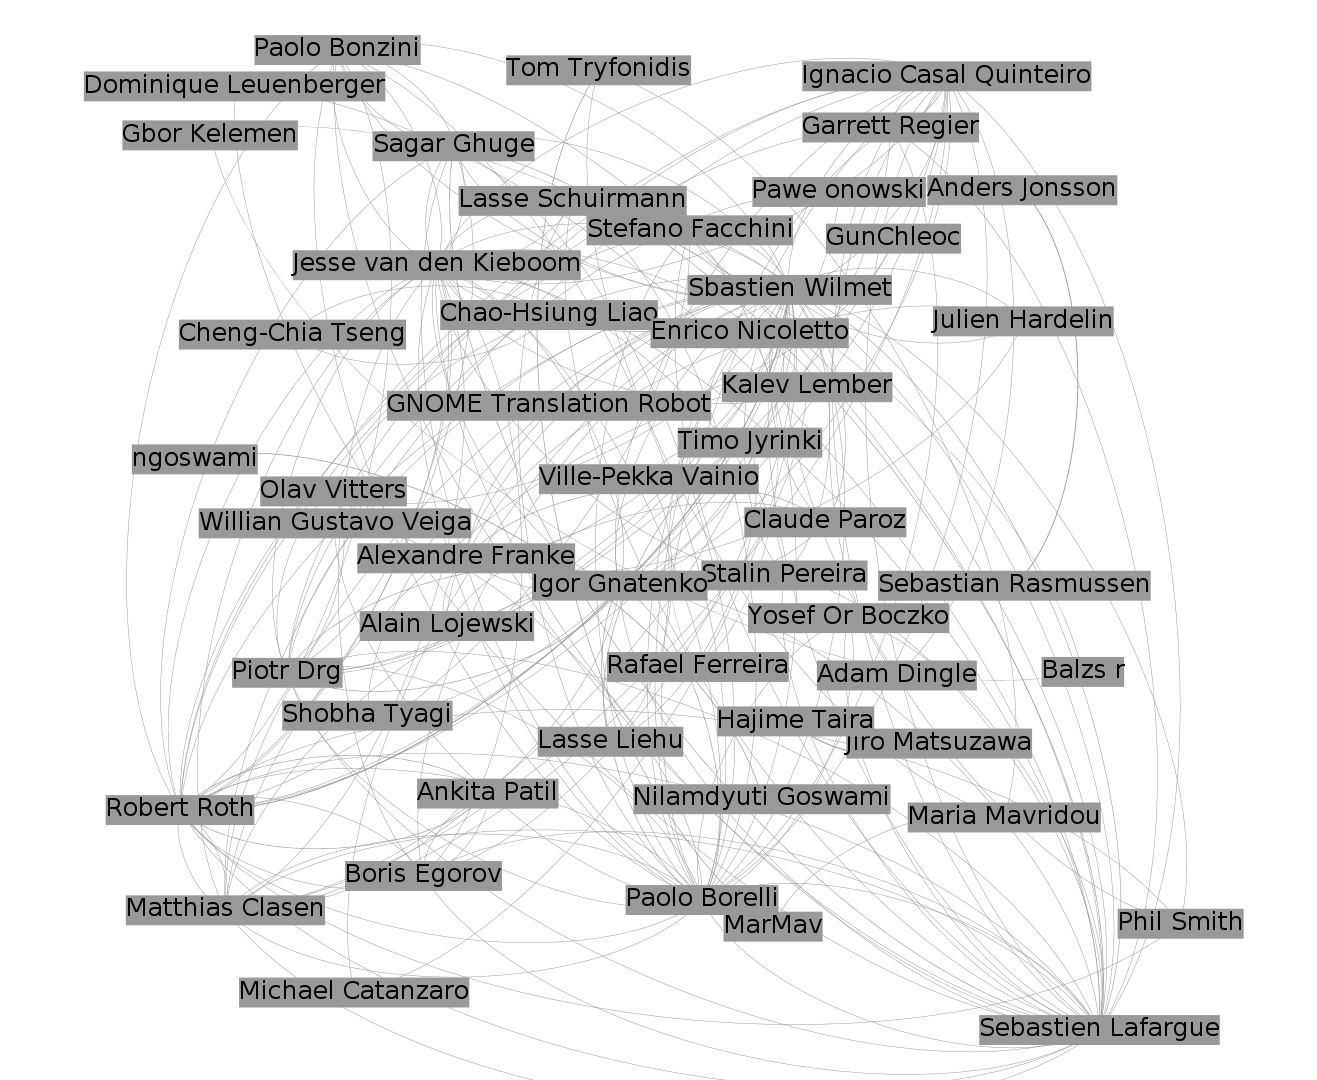
\includegraphics[scale=0.17]{g2014files.png} 
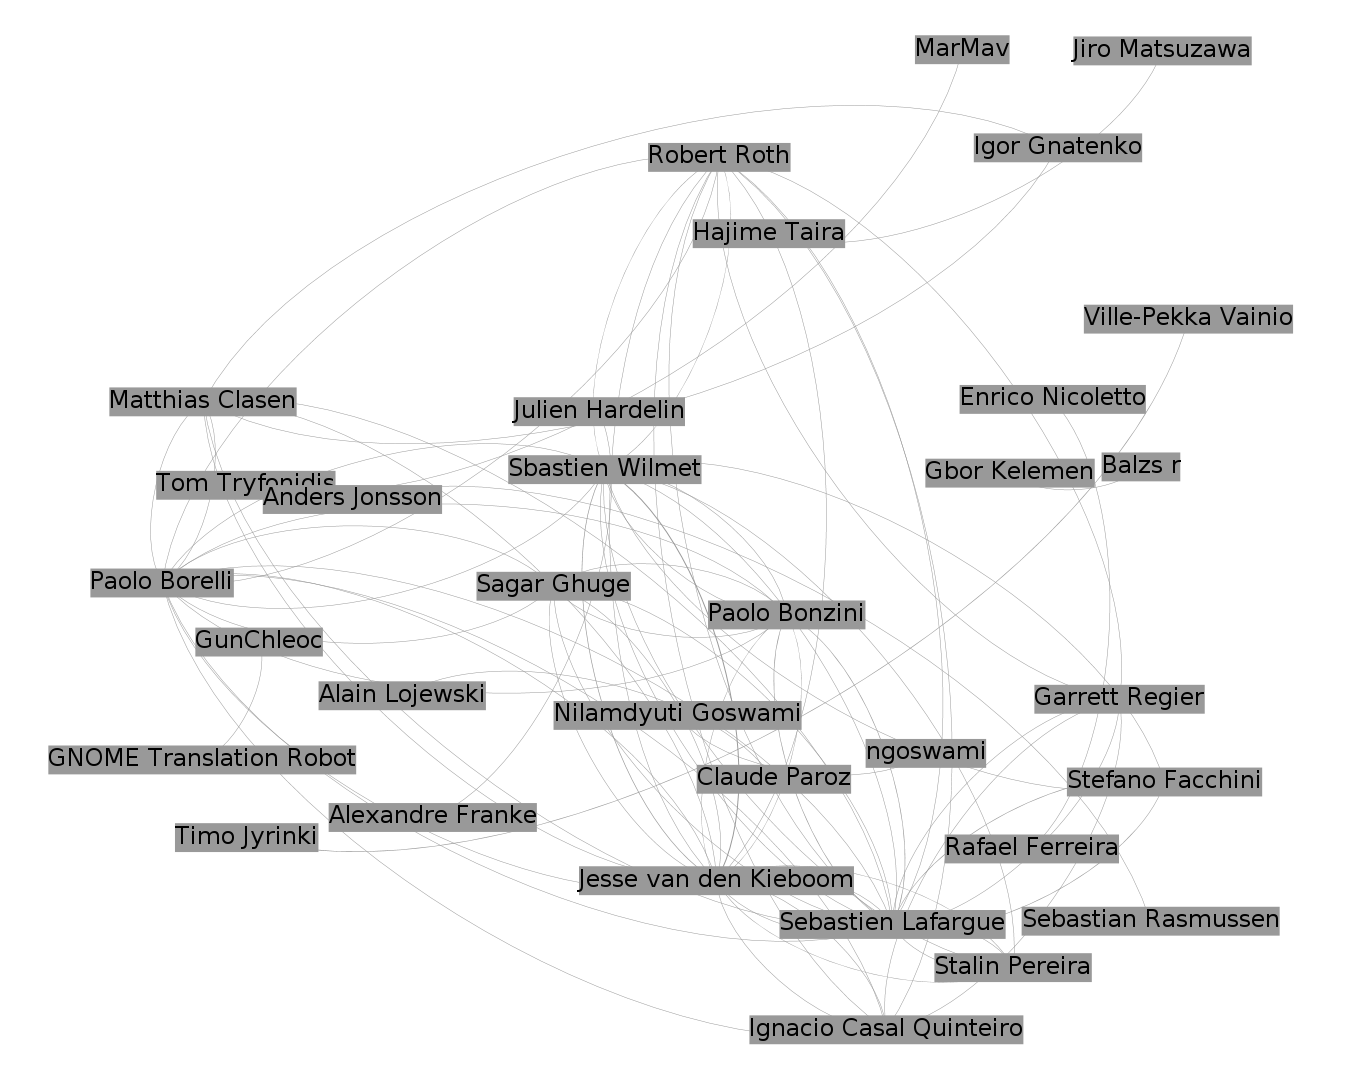
\includegraphics[scale=0.17]{g2014methods.png}
\caption{In-file (left) and In-method (right) collaboration graphs - 2014}
\label{fig:fixme2}
\end{center}
\end{figure}

\subsubsection{Numeric results}

Using Gephi, we have calculated Betweenness centrality of the resulting
graphs.
The following values are normalized [0,1], and it only appears nodes with
non-zero values.

\begin{table}[ht]
\begin{center}
\caption{Betweenness centrality from 2001-first-half data}
\bigskip

\begin{tabular}{|l|l|r|}
\hline
Node & Files & Methods\\ \hline
Jacob Leach & 0.0015873015873015873 & 0.007368421052631579\\
Jason Leach & 0.0015873015873015873 & 0.06807017543859648\\
Gediminas Paulauskas & 0.08304673721340389 & 0\\
Pablo Saratxaga & 0.10482804232804235 & 0.23964912280701753\\
Paolo Maggi & 0.12272927689594355 & 0.02140350877192982\\
Chema Celorio & 0.190189594356261 & 0.02140350877192982\\ \hline
\end{tabular}
\end{center}
\end{table}

\begin{table}[ht]
\begin{center}
\caption{Betweenness centrality from 2014-second-half data}
\bigskip

\begin{tabular}{|l|l|r|}
\hline
Node & Files & Methods\\ \hline
Igor Gnatenkov & 2.7210884353741496E-4 & 0\\
Alexandre Franke & 6.122448979591836E-4 & 0\\
Matthias Clasen & 0.008321995464852606 & 0.02217741935483871\\
Boris Egorov & 0.006448979591836735 & 0\\
Ignacio Casal Quinteiro & 0.02728312277291869 & 0.0013440860215053762\\
Piotr Drg & 0.027968901846452864 & 0\\
Jesse van den Kieboom & 0.029569160997732425 & 0.01989727342549923\\
Robert Roth & 0.030327502429543254 & 0.0041042626728110595\\
Paolo Borelli & 0.04774570780693228 & 0.012840821812596005\\
Sebastien Lafargue & 0.058611920958859746 & 0.03878648233486943\\
Sebastien Wilmet & 0.14896080336896667 & 0.00842453917050691\\ \hline
\end{tabular}
\end{center}
\end{table}



\section{Acknowledgements}

FIXME\\
Acknowledgments goes here\\

\bibliographystyle{alpha} 
\bibliography{bib}
%inline the .bbl file directly for mailing to authors.

%\begin{thebibliography}{Com79}
%
%\bibitem[Com79]{Comer-btree}
%D.~Comer.
%\newblock The ubiquitous b-tree.
%\newblock {\em Computing Surveys}, 11(2):121--137, June 1979.
%
%\bibitem[Knu73]{Knuth-vol3}
%D.~E. Knuth.
%\newblock {\em The Art of Computer Programming -- Volume 3 / Sorting and
%  Searching}.
%\newblock Addison-Wesley, 1973.
%
%\end{thebibliography}

\end{document}


